\documentclass[11pt]{amsart}
\usepackage[margin=1.15in]{geometry}
\usepackage{amsmath,amssymb,amsthm,tikz,hyperref}
\newtheorem{theorem}{Theorem}
\newtheorem{lemma}[theorem]{Lemma}
\newtheorem{corollary}[theorem]{Corollary}
\theoremstyle{remark}
\newtheorem*{remark}{Remark}
\newcommand{\Om}{\Omega}
\DeclareMathOperator{\Res}{Res}

\title{The description-tree refinement of the Gross--Witten--Wadia numerators}
\author{Vamshi Jandhyala}
\date{26 November 2026}

\begin{document}
\begin{abstract}
Voloshyn conjectured (OEIS A336110, 31 October 2026; arXiv:2609.31189, \S4.6; arXiv:2611.11670, \S3.7) that the
unsigned numerator coefficients of the large-$N$ Gross--Witten--Wadia free energy count the description trees of
type $(2,2)$ of Cori and Schaeffer by the number of leaves plus the number of internal vertices with maximal label.
We prove this for every number of edges. The proof writes a catalytic equation for the trees, solves it by the
quadratic method in a rational parametrisation, and checks that the resulting series satisfies the hypergeometric
equation that defines the numerators. The conditional interpretations recorded in OEIS A401900 follow.
\end{abstract}
\maketitle

\section{The statement}

In the large-$N$ limit of $SU(N)$ lattice gauge theory, the free energy of the Gross--Witten--Wadia model expands
into rational functions whose numerators have integer coefficients of alternating sign: $1$; $2,-2$; $5,-14,5$;
$14,-74,74,-14$; and so on (OEIS A336110). The unsigned rows add up to $1, 4, 24, 176, \dots$, the number of rooted
bridgeless planar cubic maps. That suggests the rows refine a classical map count, and Voloshyn found a refinement
that fits every computed row: a statistic on the tree encoding of these maps due to Cori and Schaeffer. A
combinatorial reading of a physics expansion is useful in both directions. It explains the integrality and
positivity of the coefficients, and it hands the counting side a statistic with a known generating function. This
note proves that the reading is right for every row.

A \emph{description tree of type $(2,2)$} \cite{CS} is a rooted plane tree with integer labels in which every leaf
has label $2$, every internal vertex $v$ other than the root has a label $\ell(v)$ with
\[
  2 \le \ell(v) \le 2 + \sum_{w \text{ child of } v} \ell(w),
\]
and the root has the largest label allowed, $2$ plus the sum of its children's labels. Call an internal vertex
\emph{maximal} when its label is the largest allowed, so the root is always maximal. For such a tree $\tau$ let
\[
  \nu(\tau) = \#\{\text{leaves}\} + \#\{\text{maximal internal vertices}\}.
\]
Let $\mathcal T_s$ be the set of these trees with $s \ge 1$ edges. Cori and Schaeffer showed that
$|\mathcal T_s| = 2^s(3s)!/((s+1)!\,(2s+1)!)$, the number of rooted bridgeless planar cubic maps with $2s$ vertices
(OEIS A000309). Put
\[
  B_s(z) = \sum_{\tau \in \mathcal T_s} z^{\nu(\tau)-2}.
\]

For $s = 2$ there are four trees (Figure~\ref{fig:s2}). The path whose middle vertex has label $2$ or $3$ has
$\nu = 2$: one leaf and the root. The path whose middle vertex has label $4$ and the cherry both have $\nu = 3$.
So $B_2(z) = 2 + 2z$. For $s = 3$ a short count gives $B_3(z) = 5 + 14z + 5z^2$.

\begin{figure}[ht]
\centering
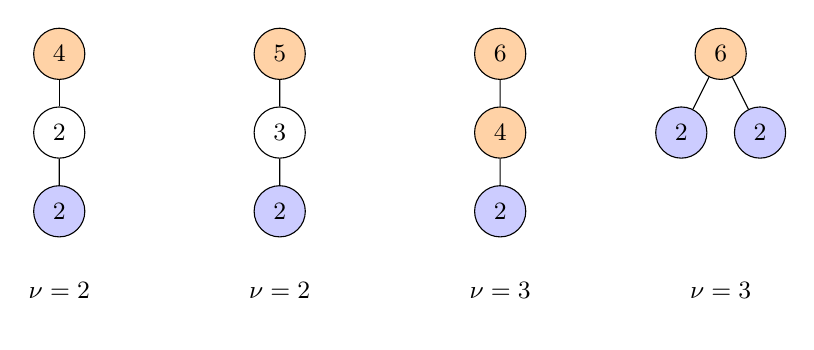
\begin{tikzpicture}[every node/.style={circle,draw,minimum size=6.5mm,inner sep=0pt,font=\small},
  level distance=10mm, sibling distance=10mm]
  \begin{scope}
    \node[fill=orange!35] {4} child {node {2} child {node[fill=blue!20] {2}}};
    \node[draw=none] at (0,-3) {$\nu=2$};
  \end{scope}
  \begin{scope}[xshift=28mm]
    \node[fill=orange!35] {5} child {node {3} child {node[fill=blue!20] {2}}};
    \node[draw=none] at (0,-3) {$\nu=2$};
  \end{scope}
  \begin{scope}[xshift=56mm]
    \node[fill=orange!35] {6} child {node[fill=orange!35] {4} child {node[fill=blue!20] {2}}};
    \node[draw=none] at (0,-3) {$\nu=3$};
  \end{scope}
  \begin{scope}[xshift=84mm]
    \node[fill=orange!35] {6} child {node[fill=blue!20] {2}} child {node[fill=blue!20] {2}};
    \node[draw=none] at (0,-3) {$\nu=3$};
  \end{scope}
\end{tikzpicture}
\caption{The four description trees of type $(2,2)$ with two edges. Leaves (blue) and maximal internal vertices
(orange) each add one to $\nu$.}
\label{fig:s2}
\end{figure}

On the other side is a triangle from mathematical physics. For $s \ge 1$ let
\[
  P_s(x) = x\,C_s\; {}_3F_2\!\left[\begin{matrix} s+\tfrac12,\ s+1,\ s+\tfrac32 \\ \tfrac12,\ \tfrac32 \end{matrix}; x^2\right]
  - x^2\, 4^s\; {}_3F_2\!\left[\begin{matrix} s+1,\ s+\tfrac32,\ s+2 \\ \tfrac32,\ 2 \end{matrix}; x^2\right],
\]
with $C_s$ the Catalan number. It is a rational function of $x$ whose denominator is a power of $1+x$ (the theorem
below shows it is $(1+x)^{3s+1}$), and A336110 lists the coefficients $T(s,n)$ of its numerator; they come from the
large-$N$ limit of $SU(N)$ lattice integrals \cite{BCV}. The rows begin $1$; $2,-2$; $5,-14,5$; $14,-74,74,-14$.

\begin{theorem}\label{thm:main}
For every $s \ge 1$,
\[
  P_s(x) = \frac{x\,B_s(-x)}{(1+x)^{3s+1}},
\]
and the fraction is in lowest terms. Equivalently, for $1 \le n \le s$,
\[
  T(s,n) = (-1)^{n-1}\,\#\{\tau \in \mathcal T_s : \nu(\tau) = n+1\}.
\]
\end{theorem}

This is the conjecture Voloshyn stated on A336110 and in \cite[\S4.6]{V1} and \cite[\S3.7]{V2}, where it was
checked for $s \le 9$ and proved for the two extreme classes $\nu = 2$ and $\nu = s+1$, each of size $C_s$. The
whole proof rests on one explicit hypergeometric term. For $k, m \ge 0$ put
\[
  \Om(k,m) = \frac{12^k}{(k+1)!\,(2k+1)!}\prod_{L=1}^{k}\binom{m+2L}{3},
\]
so that $\Om(0,m) = 1$. The theorem says, after a change of sign, that $\Om(s,m)$ is the coefficient of $z^m$ in
$z B_s(z)/(1-z)^{3s+1}$. Read this way, the coefficient of $z^m$ counts pairs (a tree $\tau$, a multiset of size
$m+1-\nu(\tau)$ drawn from $3s+1$ kinds), so the theorem is a polynomial identity in $m$ for each $s$.

\section{The proof}

The route has two halves that meet in the middle. On the tree side, the only obstacle to a recursive count is that
a vertex's allowed labels depend on its children's labels, so we keep the root label as a catalytic variable $u$
(Figure~\ref{fig:cat}). The resulting equation is quadratic in the unknown series, and Tutte's quadratic method
solves it in a rational parametrisation. On the physics side, $\Om(k,m)$ is a hypergeometric term in both indices,
so its generating function is the unique solution of a third-order differential equation with a given first row.
The proof ends by checking that the parametrised tree series satisfies that equation.

\begin{figure}[ht]
\centering
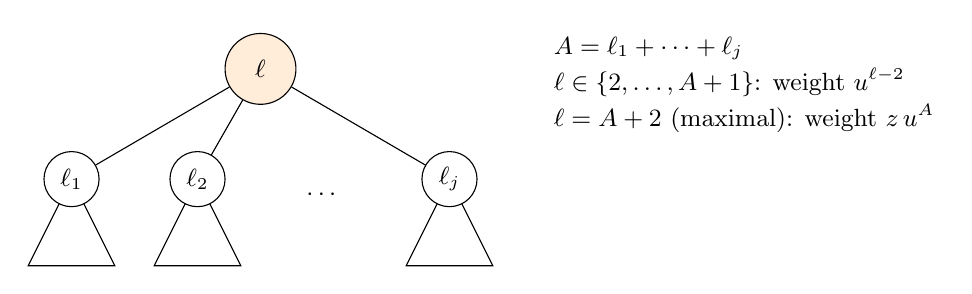
\begin{tikzpicture}[every node/.style={font=\small}]
  \node[circle,draw,minimum size=9mm,fill=orange!15] (r) at (0,0) {$\ell$};
  \foreach \x/\l in {-2.4/{\ell_1},-0.8/{\ell_2},2.4/{\ell_j}} {
    \draw (r) -- (\x,-1.4);
    \draw (\x,-1.4) -- (\x-0.55,-2.5) -- (\x+0.55,-2.5) -- cycle;
    \node[circle,draw,fill=white,minimum size=7mm,inner sep=0pt] at (\x,-1.4) {$\l$};
  }
  \node at (0.8,-1.6) {$\cdots$};
  \node[align=left,anchor=west] at (3.6,-0.2) {$A = \ell_1 + \cdots + \ell_j$\\[2pt]
    $\ell \in \{2,\dots,A+1\}$: weight $u^{\ell-2}$\\[2pt]
    $\ell = A+2$ (maximal): weight $z\,u^{A}$};
\end{tikzpicture}
\caption{A planted tree is a leaf or a root over a non-empty sequence of planted trees. The children's labels add
up to $A$, and that sum bounds the root label. Marking the root label by $u^{\ell-2}$ makes the bound visible to the
generating function: the non-maximal labels give $(1-u^{A})/(1-u)$ and the maximal one gives $zu^{A}$.}
\label{fig:cat}
\end{figure}

\subsection*{Step 1: a catalytic equation}
A \emph{planted} tree is a description tree in which the root obeys the non-root rule, so its label may be anything
from $2$ to $2$ plus the sum of its children's labels; a single vertex counts, with label $2$. Give a planted tree
the weight $t^{e}z^{\nu}u^{\ell-2}$, where $e$ is its number of edges, $\nu$ is defined as before (the root counts
only when its label is maximal) and $\ell$ is its root label. Let $P(u)$ be the sum of these weights, a power series
in $t$ whose coefficients are polynomials in $u$ and $z$, and let
\[
  Y(u) = t u^2 P(u), \qquad Q(u) = \frac{Y(u)}{1-Y(u)}.
\]
A child of label $\ell$ hangs from its parent by one edge and adds $\ell = (\ell-2)+2$ to the parent's label sum, so
$Q(u)$ counts the non-empty sequences of children, with $u$ raised to the sum of their labels. A planted tree is a
leaf, with weight $z$, or a root over such a sequence. If that sequence has label sum $A$, its root takes the labels
$2, \dots, A+1$ with weight $u^{0} + \dots + u^{A-1}$ and the maximal label $A+2$ with weight $zu^{A}$
(Figure~\ref{fig:cat}). Summing over sequences,
\begin{equation}\label{eq:cat}
  P(u) = z + \frac{Q(1)-Q(u)}{1-u} + z\,Q(u).
\end{equation}
A description tree is a root over a non-empty sequence, with its root maximal, so
$\sum_{s}\sum_{\tau\in\mathcal T_s} t^s z^{\nu(\tau)} = zQ(1)$. Hence
\[
  q := Q(1) = z\sum_{s \ge 1} B_s(z)\,t^s .
\]

\subsection*{Step 2: the quadratic method}
Write $w = 1-u$. Substituting $P = Y/(tu^2)$ and $Q = Y/(1-Y)$ in \eqref{eq:cat} and clearing denominators gives
\[
  w\,Y^2 - \bigl(w + tu^2(1+q)\bigr)Y + tu^2(zw+q) = 0 ,
\]
that is,
\[
  \bigl(2wY - A(u)\bigr)^2 = D(u), \qquad A(u) = w + tu^2(1+q), \qquad D(u) = A(u)^2 - 4w\,tu^2(zw + q).
\]
There is a unique power series $U = 1+p$ with $p \in t\,\mathbb Q[z][[t]]$ such that $2(1-U)Y(U) = A(U)$: the
condition reads $p = t(1+p)^2(1+q)/(1 - 2Y(1+p))$, a fixed-point equation whose right side is $t$ times a series.
At $u = U$ the left side of the squared equation vanishes together with its derivative in $u$, so $D(U) = D'(U) = 0$.
The resultant of $D$ and $D'$ with respect to $u$ is a polynomial combination of $D$ and $D'$, so it vanishes at
$(q,t)$. It factors as
\[
  \Res_u(D, D') = 256\,t^4\,\bigl(t(1+q)^2 - 4z\bigr)\,R(q,t),
\]
where $R$ is a polynomial of degree $4$ in $q$ with coefficients in $\mathbb Z[z,t]$ and $R(q,0) = -zq$. The middle
factor has constant term $-4z$, so $R(q,t) = 0$. Since $\partial_q R(0,0) = -z$ is invertible in $\mathbb Q(z)$,
$R$ has exactly one root in $t\,\mathbb Q(z)[[t]]$, and $q$ is that root.

Now let $p$ be defined by
\begin{equation}\label{eq:param}
  t = \frac{p(1-p)^2(1+pz)}{(1+p)^2(1-p+2pz)^2}, \qquad\text{and put}\qquad
  q_\ast = \frac{zp\bigl((1-p)^2 - 4zp^2\bigr)}{(1-p)^2(1+pz)} .
\end{equation}
Since $t = p + O(p^2)$, the first equation defines $p \in t\,\mathbb Q[z][[t]]$, and $q_\ast \in t\,\mathbb Q[z][[t]]$.
A direct computation shows $R(q_\ast, t) = 0$ as an identity in $\mathbb Q(p,z)$. By uniqueness, $q = q_\ast$.

\subsection*{Step 3: the differential equation}
Change variables to $y = t(1-z)^3$ and put
\[
  H(y,z) = \frac{z + q}{1-z} = \sum_{k \ge 0} h_k(z)\,y^k, \qquad h_k(z) = \frac{z B_k(z)}{(1-z)^{3k+1}},
\]
with $B_0 = 1$, so $h_0 = z/(1-z)$. Let $\theta_y = y\,\partial_y$ and $\theta_z = z\,\partial_z$ at fixed $y$, and let
\[
  \mathcal L = (\theta_y+1)(2\theta_y)(2\theta_y+1) - 2y\,(\theta_z+2\theta_y)(\theta_z+2\theta_y+1)(\theta_z+2\theta_y+2).
\]
Through \eqref{eq:param}, $H$ is a rational function of $p$ and $z$, and $\theta_y, \theta_z$ act on such functions
by the chain rule. (Here $p \in y\,\mathbb Q(z)[[y]]$, every denominator that occurs is nonzero at $p = 0$, and
$\partial y/\partial p = (1-z)^3 \ne 0$ at $p = 0$, so substituting the series for $p$ is an embedding of
$\mathbb Q(p,z)$ into $\mathbb Q(z)((y))$ that respects both derivations.) A direct computation shows $\mathcal L H = 0$ identically in $\mathbb Q(p,z)$. The coefficient of
$y^k$ in $\mathcal L H$ is
\[
  (k+1)(2k)(2k+1)\,h_k - 2(\theta_z+2k)(\theta_z+2k-1)(\theta_z+2k-2)\,h_{k-1} \qquad (k \ge 1),
\]
so $\mathcal LH = 0$ and $h_0$ determine every $h_k$.

The series $\sum_m \Om(k,m)z^m$ satisfy the same recurrence with the same start. Indeed
$\Om(0,m) = 1$ gives $z/(1-z)$, and $\theta_z z^m = m z^m$ together with
\[
  (k+1)(2k)(2k+1)\,\Om(k,m) = 12\binom{m+2k}{3}\Om(k-1,m) = 2(m+2k)(m+2k-1)(m+2k-2)\,\Om(k-1,m)
\]
match the recurrence term by term. Therefore, for every $k \ge 0$,
\begin{equation}\label{eq:key}
  \frac{z B_k(z)}{(1-z)^{3k+1}} = \sum_{m \ge 1} \Om(k,m)\,z^m .
\end{equation}

\subsection*{Step 4: the hypergeometric side}
\begin{lemma}\label{lem:hyp}
For $s \ge 1$ and $r \ge 0$, $\Om(s,2r+1) = C_s\,a_r$ and $\Om(s,2r+2) = 4^s b_r$, where $a_r$ and $b_r$ are the
coefficients of $X^r$ in the two ${}_3F_2$ series of $P_s$, with argument $X = x^2$.
\end{lemma}
\begin{proof}
Pair the factors: $\binom{2r+1+2L}{3} = \tfrac13 (r+L)(2r+2L-1)(2r+2L+1)$ and
$\binom{2r+2+2L}{3} = \tfrac23 (r+L)(r+L+1)(2r+2L+1)$. Taking the product over $L = 1, \dots, s$,
\[
  \Om(s,2r+1) = \frac{16^s\,(r+\frac12)_s (r+1)_s (r+\frac32)_s}{(s+1)!\,(2s+1)!}, \qquad
  \Om(s,2r+2) = \frac{16^s\,(r+1)_s (r+\frac32)_s (r+2)_s}{(s+1)!\,(2s+1)!}.
\]
On the other side, $(s+c)_r/(c)_r = (r+c)_s/(c)_s$ turns
$a_r = \frac{(s+\frac12)_r (s+1)_r (s+\frac32)_r}{(\frac12)_r (\frac32)_r\, r!}$ into
$\frac{(r+\frac12)_s (r+1)_s (r+\frac32)_s}{(\frac12)_s (\frac32)_s\, s!}$, and
$(\tfrac12)_s(\tfrac32)_s s! = (2s)!\,(2s+1)!/(16^s s!)$ gives $C_s a_r = \Om(s,2r+1)$. In the same way
$b_r = \frac{(r+1)_s (r+\frac32)_s (r+2)_s}{s!\,(\frac32)_s\,(s+1)!}$ and $(\tfrac32)_s = (2s+1)!/(4^s s!)$ give
$4^s b_r = \Om(s,2r+2)$.
\end{proof}

\subsection*{Step 5: conclusion}
By Lemma~\ref{lem:hyp}, $P_s(x) = \sum_{m\ge1} (-1)^{m+1}\Om(s,m)\,x^m$. Put $z = -x$ in \eqref{eq:key}:
\[
  P_s(x) = -\sum_{m \ge 1}\Om(s,m)(-x)^m = \frac{x\,B_s(-x)}{(1+x)^{3s+1}} .
\]
At $x = -1$ the numerator equals $-B_s(1) = -|\mathcal T_s| \ne 0$, so the fraction is in lowest terms and its
numerator is $\sum_n T(s,n)x^n$. Comparing coefficients of $x^n$ gives
$T(s,n) = (-1)^{n-1}[z^{n-1}]B_s(z)$, which is Theorem~\ref{thm:main}. \qed

\section{Consequences}

\begin{corollary}\label{cor:a401900}
Let $D_n(x) = (1-x)^{3n+1}\sum_{r \ge 0}\Pi_n(r)x^r$ with
$\Pi_n(r) = 4^n (r+\frac12)_n (r+1)_n (r+\frac32)_n/(n!\,(\frac32)_n\,(n+1)!)$, the polynomial whose coefficients
form OEIS A401900, for $n \ge 1$. Then, for $k \ge 0$, $[x^k]D_n(x)$ is the number of
pairs $(\tau, M)$ with $\tau \in \mathcal T_n$ and $M$ a subset of a fixed set of $3n+1$ elements such that
$\nu(\tau) - 2 + |M| = 2k$.
\end{corollary}
\begin{proof}
Voloshyn proved the identity $(1+z)^{3n+1}B_n(z) = D_n(z^2) + 4^n z E_n(z^2)$, with $B_n$ the unsigned A336110
row and $E_n$ the A140136 row \cite[eq.~(64)]{V1}, so $D_n(z^2)$ is the even part of $(1+z)^{3n+1}B_n(z)$, and he
noted that the pair count would follow from the tree refinement. Theorem~\ref{thm:main} supplies that refinement:
expanding $(1+z)^{3n+1}$ as a sum over subsets $M$ gives the count. For completeness, the even-part statement also
follows directly from \eqref{eq:key}. Since $(\frac32)_n = (2n+1)!/(4^n n!)$, $\Pi_n(r) = \Om(n,2r+1)$ by the first display in the proof of
Lemma~\ref{lem:hyp}. Write $F(z) = zB_n(z)/(1-z)^{3n+1}$. By \eqref{eq:key} the odd part of $F$ is
$\sum_r \Om(n,2r+1) z^{2r+1}$. Multiplying $\tfrac12(F(z)-F(-z))$ by $(1-z^2)^{3n+1}$ gives
\[
  z\,D_n(z^2) = \tfrac{z}{2}\Bigl((1+z)^{3n+1}B_n(z) + (1-z)^{3n+1}B_n(-z)\Bigr).
\]
The right side is $z$ times the even part of $(1+z)^{3n+1}B_n(z)$.
\end{proof}

So the interpretation that Voloshyn \cite[\S4.6]{V1} and A401900 record as conditional is unconditional. Two remarks on what remains. First, the
proof is not bijective. Voloshyn asks for a path bijection, and the pair count in Corollary~\ref{cor:a401900} still
lacks a local meaning for the $3n+1$ elements. Second, the parametrisation \eqref{eq:param} is rational in $p$ and
$z$ together, and it may be the natural place to look for one. At $z = 1$ it reads $t = p(1-p)^2/(1+p)^3$ and
$q = p(1-3p)/(1-p)^2$.

\section*{Verification and AI use}
The computations in Steps 2 and 3 (the resultant and its factorisation, $R(q_\ast,t) = 0$, and $\mathcal L H = 0$)
are exact rational-function identities checked with SymPy. The accompanying scripts also check, for finitely many
cases only, the catalytic equation against a brute-force enumeration of the trees ($s \le 9$) and \eqref{eq:key}
against the same enumeration ($s \le 12$); the general statements rest on the argument above. The
identities of Lemma~\ref{lem:hyp}, the recurrence and uniqueness step of Step~3, and the identity $R(q_\ast,t)=0$
are also checked in Lean~4 with Mathlib; the code is in the archive listed below.

Claude Opus 5.5 (Anthropic) found the proof, wrote the scripts and the Lean code, and drafted the text. Codex
(OpenAI) ran an independent literature search and an independent check of every step; it found a sign error in the
displayed resultant, now corrected, and wrote a recheck program that shares no code with the others. The author
directed the work and is responsible for the result. Code and data:
\url{https://github.com/jvvk/mathematics/tree/main/description-tree-refinement}; archived at
\href{https://doi.org/10.5281/zenodo.24561485}{doi:10.5281/zenodo.24561485}.

\begin{thebibliography}{9}
\bibitem{BCV} O.~Borisenko, V.~Chelnokov and S.~Voloshyn, \emph{The large $N$ limit of $SU(N)$ integrals in lattice
models}, arXiv:2008.00773 (2020), eq.~(48).
\bibitem{CS} R.~Cori and G.~Schaeffer, \emph{Description trees and Tutte formulas}, Theoret. Comput. Sci. 292 (2003),
165--183.
\bibitem{V1} S.~Voloshyn, \emph{Differential recursions, projective discriminants, and algebraic generating
functions}, arXiv:2609.31189v3 (2026), \S4.6.
\bibitem{V2} S.~Voloshyn, \emph{Projective symmetries and differential recursions for the large-$N$
Gross--Witten--Wadia and one-dimensional QCD matrix models}, arXiv:2611.11670 (2026), \S3.7.
\bibitem{OEIS} OEIS Foundation, sequences A000309, A336110, A401900, \url{https://oeis.org}.
\end{thebibliography}
\end{document}
